\documentclass{standalone}
\usepackage{tikz}
\usepackage{color}

\begin{document}
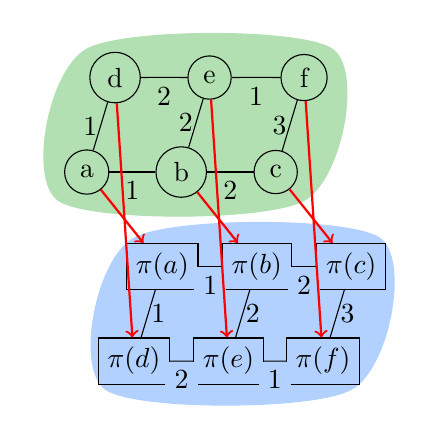
\begin{tikzpicture}[scale=1.2]
\definecolor{mycolor1}{HTML}{009900}
\definecolor{mycolor2}{HTML}{0066FF}
\draw[draw=mycolor1!30, fill=mycolor1!30] plot[smooth cycle, tension=0.5] coordinates
{(-0.3, -0.3) (2.3,-0.3) (2.6, 1.3) (-0.0,1.3)};

\node[draw,circle] (0_00) at (0,0) {a};
\node[draw,circle] (0_01) at (0.3,1) {d};
\node[draw,circle] (0_10) at (1,0) {b};
\node[draw,circle] (0_11) at (1.3,1) {e};
\node[draw,circle] (0_20) at (2,0) {c};
\node[draw,circle] (0_21) at (2.3,1) {f};

\draw (0_00) -- (0_01) node [inner sep=0pt, midway, xshift = -1pt, left, fill=mycolor1!30] {1};
\draw (0_10) -- (0_11) node [inner sep=0pt, midway, xshift=-1pt, left, fill=mycolor1!30] {2};
\draw (0_20) -- (0_21) node [inner sep=0pt, midway, midway, xshift=-1pt, left, fill=mycolor1!30] {3};
\draw (0_00) -- (0_10) node [midway, below, fill=mycolor1!30] {1};
\draw (0_10) -- (0_20) node [midway, below, fill=mycolor1!30] {2};
\draw (0_01) -- (0_11) node [midway, below, fill=mycolor1!30] {2};
\draw (0_11) -- (0_21) node [midway, below, fill=mycolor1!30] {1};

\draw[draw=mycolor2!30, fill=mycolor2!30] plot[smooth cycle, tension=0.5] coordinates
{(-0.3+0.5, -2-0.3) (0.5+2.3,-2-0.3) (0.5+2.6, -2+1.3) (0.5+-0.0,-2+1.3)};

\node[draw,rectangle] (1_00) at (0+0.5,-2) {$\pi(d)$};
\node[draw,rectangle] (1_01) at (0.3+0.5,-2+1) {$\pi(a)$};
\node[draw,rectangle] (1_10) at (1+0.5,-2) {$\pi(e)$};
\node[draw,rectangle] (1_11) at (1.3+0.5,-2+1) {$\pi(b)$};
\node[draw,rectangle] (1_20) at (2+0.5,-2) {$\pi(f)$};
\node[draw,rectangle] (1_21) at (2.3+0.5,-2+1) {$\pi(c)$};

\draw (1_00) -- (1_01) node [inner sep=0pt, midway, xshift=1pt, right, fill=mycolor2!30] {1};
\draw (1_10) -- (1_11) node [inner sep=0pt, midway, xshift=1pt, right, fill=mycolor2!30] {2};
\draw (1_20) -- (1_21) node [inner sep=0pt, midway, xshift=1pt, right, fill=mycolor2!30] {3};
\draw (1_00) -- (1_10) node [midway, below, fill=mycolor2!30] {2};
\draw (1_10) -- (1_20) node [midway, below, fill=mycolor2!30] {1};
\draw (1_01) -- (1_11) node [midway, below, fill=mycolor2!30] {1};
\draw (1_11) -- (1_21) node [midway, below, fill=mycolor2!30] {2};

\draw[->,red,thick] (0_00) -- (1_01);
\draw[->,red,thick] (0_01) -- (1_00);
\draw[->,red,thick] (0_10) -- (1_11);
\draw[->,red,thick] (0_11) -- (1_10);
\draw[->,red,thick] (0_20) -- (1_21);
\draw[->,red,thick] (0_21) -- (1_20);

\end{tikzpicture}
\end{document}
